\section{Background} \label{sec:background}

\subsection{KVM} \label{sec:kvm}

KVM is a more recent hypervisor which embeds virtualization capabilities 
in Linux kernel using x86 hardware virtualization extensions~\cite{kivity2007kvm}. 
It is a full virtualization solution, where guests are run unmodified in VMs. 

Figure 1 shows the typical KVM architecture, with reference to a network related
application. 

As depicted in the picture, when a packet arrives at physical NIC,
interrupts generated by NIC are handled by the physical device driver. The device
driver forwards the packet to software bridge. The bridge, then pushes the packet
to the tap device of the corresponding VM. The tap device is a virtual network
device that sends a signal to KVM module. KVM module in turn, generates a virtual
interrupt to the user space Qemu of the target VM. Qemu then copies the packet from
tap device and generates the interrupt for the guest OS emulating the virtual NIC.
Again, the physical device driver in the guest OS handles the packet transfer to
the VM’s address space. A major advantage of the KVM architecture is the full
availability of user-space tools in the QEMU process, such as threading, libraries
and so on.

\begin{figure}[t]
% \vspace{.20in}
\centering
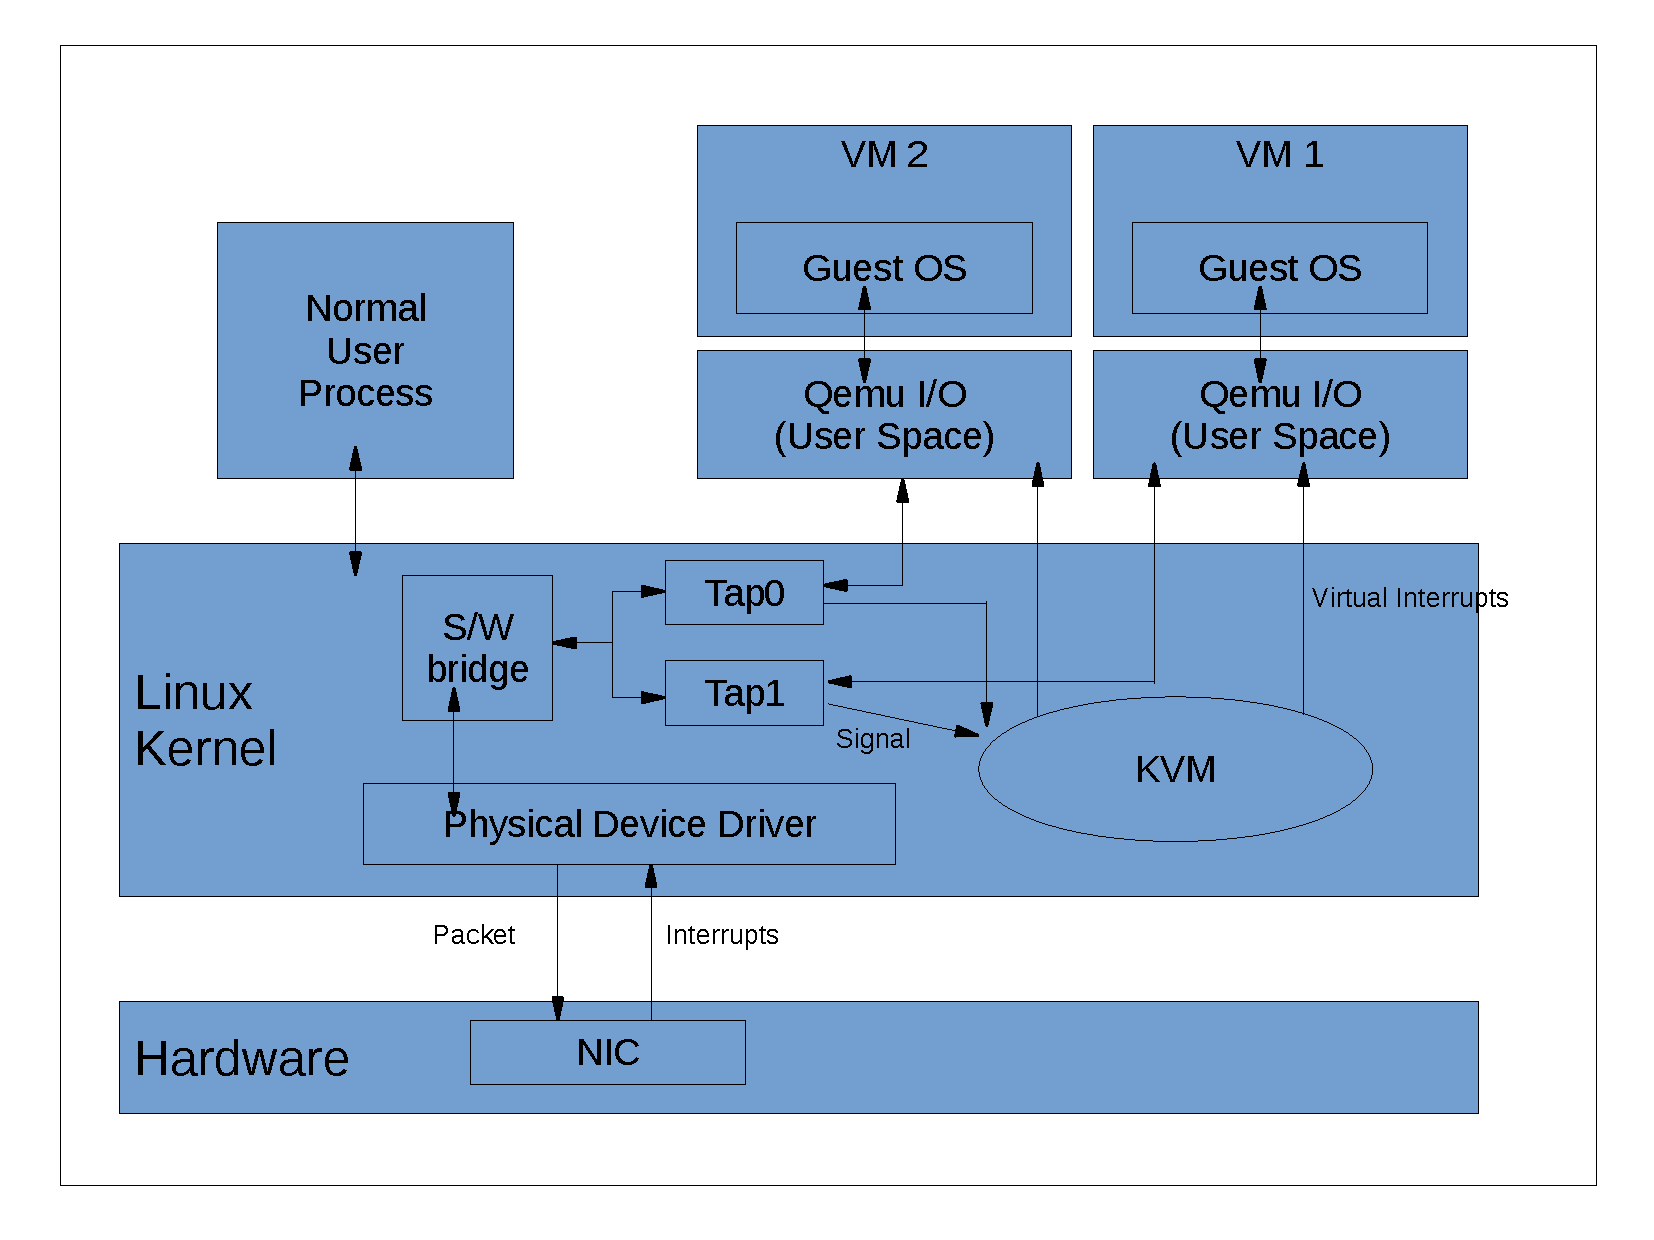
\includegraphics[width=.47\textwidth]{figures/kvm}
\vspace{-.2in}
\caption{{\em KVM Architecture.}} \label{fig:kvm}
\vspace{.05in}
\end{figure}

\subsection{FALCON} \label{sec:falcon}

\smrsystem is an \smr system that replicates general server programs efficiently. On 
receiving a client network request, it invokes a RDMA-based consensus process on this 
request to enforce that all replicas see the same sequence of input requests. 

Unlike previous \smr systems which either reply on deterministic multithreading and replay
approach~\cite{rex:eurosys14} or manually annotate all shared states~\cite{eve:osdi12}, 
\smrsystem deals with non-determinism at low overhead and automatically. It captures the 
network outputs of the programs to compute an accumulated hash value. The leader collects 
the corresponding hash values from other nodes occasionally to detect divergence of execution 
states across replicas.
